

\section{GIỚI THIỆU ĐỀ TÀI}

\subsection{Mô tả bài toán nhận diện chứng minh nhân dân}
Trong cuộc cách mạng công nghệ ngày nay, để đăng kí sử dụng một dịch vụ, thay vì bắt người dùng phải điền thông tin cá nhân vào những biểu mẫu rườm rà thì các công ty có thể tự động trích xuất các thông tin từ chứng minh nhân dân của người dùng đó. Hệ thống này giúp tiết kiệm thời gian cho cả người dùng và doanh nghiệp. Tất cả những gì người dùng cần làm là chụp ảnh chứng minh nhân dân của mình, hệ thống sẽ tự động trích xuất thông tin từ ảnh được người dùng nhập vào. Trong đó, bước đầu tiên của hệ thống là phát hiện chính xác chứng minh nhân dân trong ảnh và biến đổi nó về dạng "thẳng", phục vụ các bước trích xuất thông tin về sau. \\

\begin{figure}[h]
\centering
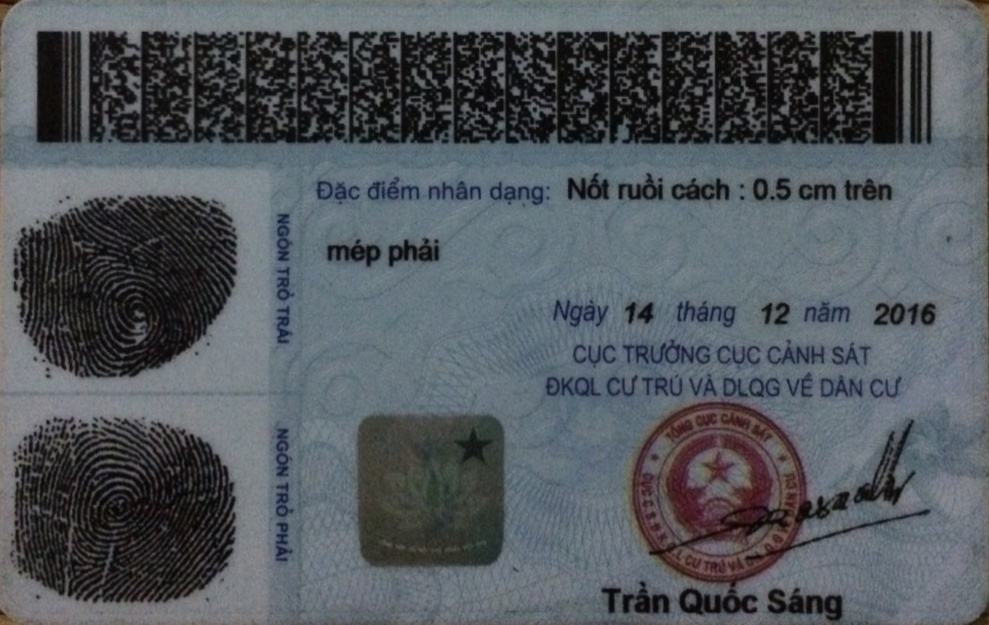
\includegraphics[scale=0.3]{../figure/1.jpg}
\caption{abc}
\end{figure}

Để làm tốt bước này, mô hình phát hiện chứng minh nhân dân cần phải giải quyết những vấn đề phát sinh trong thực tế sau:
\begin{itemize}
\item Chứng minh nhân dân từ ảnh chụp của người dùng có thể bị xoay nghiêng, lật ngược, méo mó, quăn góc, ...
\item Người dùng chụp ảnh có thể xén mất góc của chứng minh nhân dân, dẫn đến việc các trường thông tin có thể bị mất mát. Mô hình cần nhận diện các trường hợp này và thông báo cho người dùng để cung cấp ảnh mới.
\end{itemize}

\subsection{Phương pháp truyền thống}

